\label{key}\documentclass[UTF8,a4paper,11pt]{ctexart}
\usepackage[left=2.50cm, right=2.50cm, top=2.50cm, bottom=2.50cm]{geometry} %页边距
\CTEXsetup[format={\Large\bfseries}]{section} 
 

% compile using Xelatex
%%%%%%%%%%%%%%%%%%%%%%%   字体备选栏
% -- 中文字体 --
%\setmainfont{Microsoft YaHei}  % 微软雅黑
%\setmainfont{YouYuan}  % 幼圆    
%\setmainfont{NSimSun}  % 新宋体
%\setmainfont{KaiTi}    % 楷体
%\setmainfont{SimSun}   % 宋体
%\setmainfont{SimHei}   % 黑体
% -- 英文字体 --
%\usepackage{times}
%\usepackage{mathpazo}
%\usepackage{fourier}
%\usepackage{charter}
\usepackage{helvet}
 
\usepackage{amsmath, amsfonts, amssymb} % math equations, symbols
\usepackage[english]{babel}
\usepackage{color}      % 控制文本颜色
\usepackage{graphicx}   % 加载图像包
\usepackage{url}        % 网址超链接
\usepackage{bm}         % equations的粗体形式
\usepackage{tikz}       % tikz 图像包
\usepackage{multirow}	% 列表设置一格多行多列
\usepackage{ulem}
\usepackage{booktabs}
\usepackage{epstopdf}
\usepackage{epsfig}
\usepackage{algorithm}  %编写算法

\usepackage{hyperref} %此处设置文本内超链接

%\usepackage{CJK,pgf,pgfarrows,pgfnodes,pgfautomata,pgfheaps}
\usepackage{amsmath,amssymb}
\usepackage{geometry}%页面设置
\usepackage{graphicx}%图片设置
\usepackage{float} %指定图片位置
%\usepackage{subfig}%多个子图
\usepackage{subfigure}%并排子图 共享标题 有子标题
\usepackage{caption}%注释设置

\usepackage{algorithm}
\usepackage{algorithmicx}
\usepackage{algpseudocode}  

% 这个和algorithmic不兼容,用了就要报错,好多莫名其妙的错误!!!!!
\floatname{algorithm}{算法}  
\renewcommand{\algorithmicrequire}{\textbf{输入:}}  
\renewcommand{\algorithmicensure}{\textbf{输出:}}  
\renewcommand{\algorithmicrequire}{ \textbf{Input:}}     %Use Input in the format of Algorithm
\renewcommand{\algorithmicensure}{ \textbf{Output:}}    %UseOutput in the format of Algorithm

\newtheorem{pf}{Pf}
\newtheorem{sol}{Sol}[section]
\newtheorem{thm}{Thm}
% 算法示例备选项
%\renewcommand{\algorithmicrequire}{ \textbf{Input:}}     % use Input in the format of Algorithm  
%\renewcommand{\algorithmicensure}{ \textbf{Initialize:}} % use Initialize in the format of Algorithm  
%\renewcommand{\algorithmicreturn}{ \textbf{Output:}}     % use Output in the format of Algorithm  

\DeclareMathOperator{\dif}{d\!}  %定义微分的缩写
\DeclareMathOperator{\pa}{\partial}  %定义偏微分的缩写

%\usepackage{fancyhdr}  %这里对 页眉、页脚 进行设置
%\pagestyle{fancy}
%\rhead{\thepage}
%\chead{}
%%\lhead{\includegraphics[width=1.6cm]{wallpaper.jpg}}
%\lfoot{}
%\cfoot{Page \thepage{} of \pageref{LastPage}}
%\rfoot{}
%
%\newcommand{\makeheadrule}{%        %去除页眉的横线 以免遮挡后面文字 
%	\makebox[0pt][l]{\rule[0\baselineskip]{\headwidth}{0pt}}%
%	\rule[0\baselineskip]{\headwidth}{0pt}}
%\renewcommand{\headrule}{%
%	{\if@fancyplain\let\headrulewidth\plainheadrulewidth\fi
%		\makeheadrule}}

%\usepackage[printwatermark]{xwatermark}   %%这以下设置“数学外卖”官方水印
%\usepackage{lipsum}
%
%\newsavebox\mybox
%
%\savebox\mybox{\tikz[color=gray,opacity=0.3]
%\newwatermark*[
%allpages,
%angle=48,
%scale=6,
%xpos=-20,
%ypos=15
%]{\usebox\mybox} 
 


\title{\textbf{Homework 2}}
\author{ 张思源  \qquad  \textit{21110850018} }   %这里填上您的大名


\begin{document}
\maketitle
\section{Ex1}
\textbf{使用波士顿房价数据集,以线性回归为例(或者自行设定模型)实现以及对比梯度下降方式:随机梯度下降、牛顿法、Adagrad.\\
NOTE:1.需要附有梯度下降表达式.2.列表对比三种方法的区别.}
\begin{sol}
	首先计算梯度,在此之前计算MSE函数表达式为:
	$$
	MSE=\frac{1}{n}\sum_{i=1}^{n}(w^{T}x_{i}+b-y_{i})^{2}
	$$
	其中$n$为样本数,在此基础上,计算其梯度为:
	\begin{equation*}
		\begin{split}
			\nabla_{w} MSE&=\frac{2}{n}\sum_{i=1}^{n}(w^{T}x_{i}+b-y_{i})x_{i}\\
			\nabla_{b} MSE&=\frac{2}{n}\sum_{i=1}^{n}(w^{T}x_{i}+b-y_{i})
		\end{split}
	\end{equation*}
	更进一步的,其Hessian矩阵为:
	\begin{equation*}
		\begin{split}
			H(w)&=\frac{2}{n}X^{T}X\\
			H(b)&=\frac{2}{n}I
		\end{split}
	\end{equation*}
因此,三种优化方法的迭代公式为(为了简便表示,记参数为$\theta=(w,b)$):
\begin{itemize}
	\item SGD的迭代表达式为:$$\theta_{t+1} \leftarrow \theta_{t}-\eta \nabla MSE_{i},$$其中$\eta$为学习率,$MSE_{i}$为随机样本的MSE函数.
	\item AdaGrad算法会使用一个小批量随机梯度 $\boldsymbol{g}_{t}$ 按元素平方的累加变量 $\boldsymbol{s}_{t} $.在时间步0, AdaGrad将 $\boldsymbol{s}_{0}$ 中每个元素初始化为 0 .在时间步 $t$, 首先将小批量随机梯度 $\boldsymbol{g}_{t}$ 按元素 平方后累加到变量 $\boldsymbol{s}_{t}$ :
	$$
	\boldsymbol{s}_{t} \leftarrow \boldsymbol{s}_{t-1}+\boldsymbol{g}_{t} \odot \boldsymbol{g}_{t}
	$$
	其中$\odot$ 是按元素相乘.接着,我们将目标函数自变量中每个元素的学习率通过按元素运算重新调整一下:
	$$
	\theta_{t+1} \leftarrow \theta_{t}-\frac{\eta}{\sqrt{s_{t}+\epsilon}} \odot \boldsymbol{g}_{t}
	$$
	其中 $\eta$ 是学习率,$\epsilon$ 是为了维持数值稳定性而添加的常数,如 $10^{-6}$ .这里开方、除法和乘法的运算都是按元素运算的.这些按元素运算使得目标函数自变量中每个元 素都分别拥有自己的学习率.
	\item Newton法的迭代表达式为:$$\theta_{t+1} \leftarrow \theta_{t}-H^{-1}\nabla MSE.$$这里$H$为Hessian矩阵.
\end{itemize}
而数值实验的结果如下图所示:
\begin{figure}[H]
	\centering
	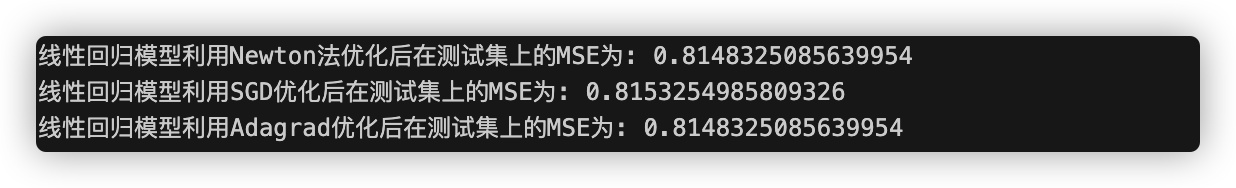
\includegraphics[width=0.9\textwidth,height=0.2\textwidth]{result.png}
	\caption{Results of 3 different methods of optimization}
\end{figure}
接下来,比较三种不同的优化方法:\\
\begin{center}
	\begin{tabular}{c p{5cm} p{5cm}}
	
	\hline
	算法 & 优点 & 缺点 \\
	\hline
	SGD &计算速度快,计算成本低  & 1.选择合适的learning rate比较困难,对所有的参数更新使用同样的learning rate.2.容易收敛到局部最优,并且在某些情况下可能被困在鞍点.\\

	Adagrad & 前期$g_{t}$较小的时候,regularizer较大,能够放大梯度;后期$g_{t}$较大的时候,regularizer较小,能够约束梯度.适合处理稀疏梯度. & 1.$\eta$设置过大的话,会使regularizer过于敏感,对梯度的调节太大
	2.中后期,分母上梯度平方的累加将会越来越大,使$g_{t}\rightarrow 0$,使得训练提前结束.
	\\

	Newton & 收敛速度快,二阶方法精确度高 & 1.容易收敛到鞍点2.计算逆矩阵容易出现数值不稳定 \\
	\hline
\end{tabular}
\end{center}

\end{sol}
\newpage
\section{Ex2}
\textbf{分别使用误差率,信息熵,基尼指数来计算计算下图不纯度.哪个不纯度最高?哪个不纯度最低?}
\begin{figure}[H]
	\centering
	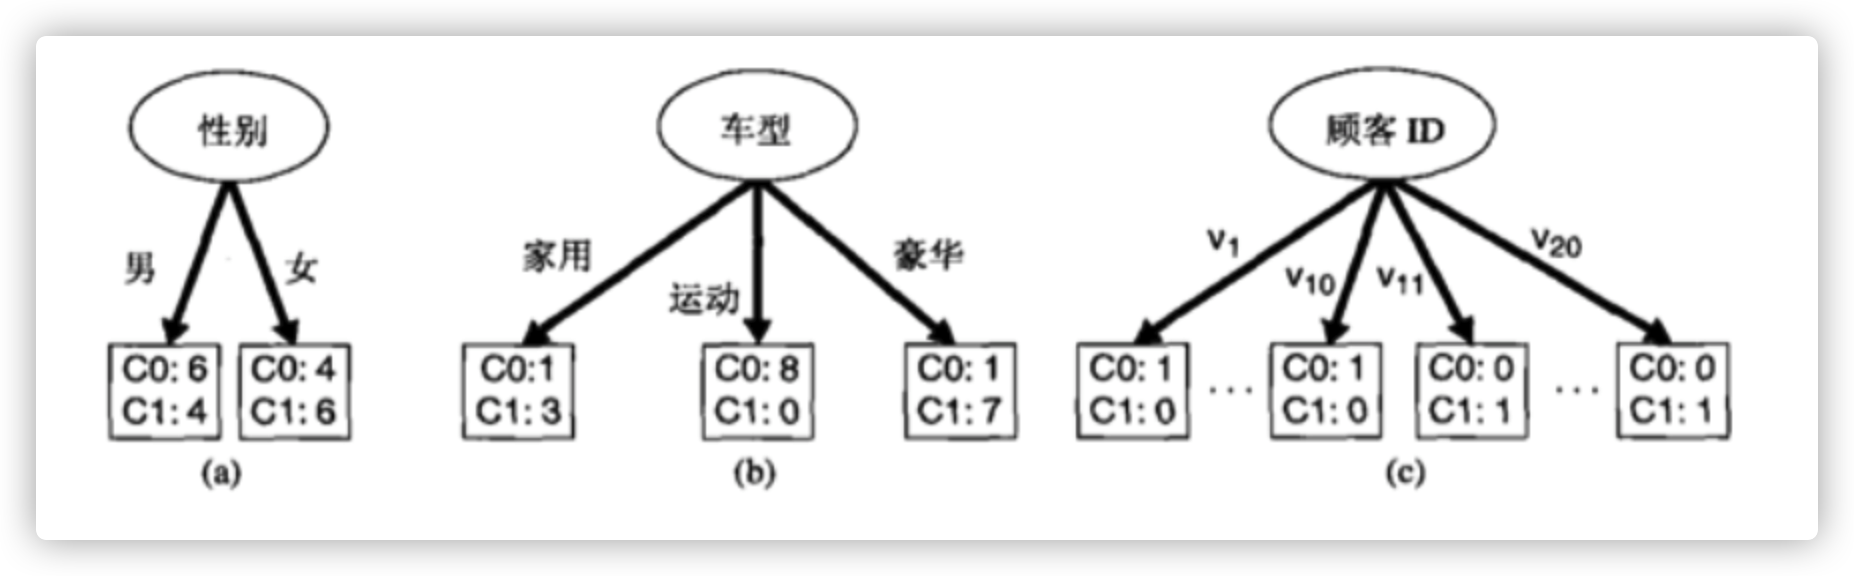
\includegraphics[width=0.8\textwidth,height=0.4\textwidth]{Ex2.png}
	\caption{Ex2}
\end{figure}
\begin{sol}
	在计算中,以$Ce$表示误差率,以$Entropy$表示信息熵,以$Gini$表示基尼系数.\\
	则对$(a)$图,注意到两个节点的对称性,有:
	\begin{equation*}
		\begin{split}
			Ce(a)&=1-\max(0.4,0.6)=0.4\\
			Entropy(t_{1})&=-(0.4\times \log_{2}0.4+0.6\times\log_{2}0.6)=0.9710=Entropy(t_{2})\\
			Entropy(a)&=\frac{6+4}{20}Entropy(t_{1})+\frac{4+6}{20}Entropy(t_{2})=0.9710\\
			Gini(t_{1})&=1-(0.6^{2}+0.4^{2})=0.48=Gini(t_{2})\\
			Gini(a)&=\frac{6+4}{20}Gini(t_{1})+\frac{4+6}{20}Gini(t_{2})=0.48
		\end{split}
	\end{equation*}
对图$(b)$,有:
\begin{equation*}
	\begin{split}
		Ce(b)&=1-\max(0.75,0,0.875)=0.125\\
		Entropy(t_{1})&=-(0.25\times\log_{2}0.25+0.75\times\log_{2}0.75)=0.8113\\
		Entropy(t_{2})&=-(1\times\log_{2}1+0\times\log_{2}0)=0\\
		Entropy(t_{3})&=-(0.125\times\log_{2}0.125+0.875\times\log_{2}0.875)=0.5436\\
		Entropy(b)&=\frac{1+3}{20}Entropy(t_{1})+\frac{8+0}{20}Entropy(t_{2})+\frac{1+7}{20}Entropy(t_{3})=0.3797\\
		Gini(t_{1})&=1-(0.25^{2}+0.75^{2})=0.375\\
		Gini(t_{2})&=1-(1^{2}+0^{2})=0\\
		Gini(t_{3})&=1-(0.125^{2}+0.875^{2})=0.21875\\
		Gini(b)&=\frac{1+3}{20}Gini(t_{1})+\frac{8+0}{20}Gini(t_{2})+\frac{1+7}{20}Gini(t_{3})=0.1625
	\end{split}
\end{equation*}
对图$(c)$,同样注意到对称性,有:
\begin{equation*}
	\begin{split}
		Ce(c)&=1-\max(0,\dots,0,1,\dots,1)=0\\
		Entropy(t_{i})&=-(1\times\log_{2}1+0\times\log_{2}0)=0,i=1,2,\dots,10\\
		Entropy(t_{j})&=-(0\times\log_{2}0+1\times\log_{2}1)=0,j=11,12,\dots,20\\
		Entropy(c)&=\sum_{i=1}^{20}\frac{1}{20}Entropy(t_{i})=0\\
		Gini(t_{i})&=1-(1^{2}+0^{2})=0,i=1,2,\dots,10\\
		Gini(t_{j})&=1-(0^{2}+1^{2})=0.j=11,12,\dots,20\\
		Gini(c)&=\sum_{i=1}^{20}\frac{1}{20}Gini(t_{i})=0
	\end{split}
\end{equation*}
\end{sol}
故有:
\begin{equation*}
	\begin{split}
		&Ce(a)=0.4>Ce(b)=0.125>Ce(c)=0\\
		&Entropy(a)=0.9710>Entropy(b)=0.3797>Entropy(c)=0\\
		&Gini(a)=0.48>Gini(b)=0.1625>Gini(c)=0
	\end{split}
\end{equation*}
即图$(a)$的不纯度最大,图$(c)$的不纯度最小.
\newpage
\begin{thebibliography}{3}  
	\bibitem{ref1} 李航. 统计学习方法[M]. 清华大学出版社, 2012.
	%\bibitem{ref2} Kingma D , Ba J . Adam: A Method for Stochastic Optimization[J]. Computer Science, %2014.
	\bibitem{ref2} Goodfellow, Ian, et al. Deep Learning[M]. MIT Press, 2016. 	
\end{thebibliography}
\end{document}
